\documentclass[11pt,a4paper]{article}
\usepackage[margin=1in, headheight=14pt]{geometry}
\usepackage{amsfonts,amsmath,amssymb,suetterl}
\usepackage{lmodern}
\usepackage[T1]{fontenc}
\usepackage{fancyhdr}
\usepackage{float}
\usepackage[utf8]{inputenc}
\usepackage{fontawesome}
\usepackage{enumerate}
\usepackage{xcolor}
\usepackage{hyperref}
\usepackage{tikz}
\usepackage{nicefrac}
\usepackage{subcaption}
\usepackage{physics}
\usepackage{mathtools}
\usepackage{adjustbox}

\DeclareUnicodeCharacter{2212}{-}

\usepackage{mathrsfs}
\usepackage[nodisplayskipstretch]{setspace}

\setstretch{1.5}
\renewcommand{\footrulewidth}{0pt}

\parindent 0ex
\setlength{\parskip}{1em}
\raggedbottom

\begin{document}
  %
	\begin{center}
		\vspace*{8cm}
		\Huge MA202 –Differential Equations\\
		\LARGE LECTURE 17
  \end{center}
  \newpage
  %
	\section*{Examples of nonlinear systems}
	\subsection*{Population dynamics: Competing species}
	\begin{itemize}
		\item Here we will explore the application of phase plane analysis to some problems in population dynamics.
		\item These problems involve two interacting populations and are extensions of those discussed in week 1, which dealt with a single population.
		\item Although the relationships discussed here are overly simple compared to the complex relationships in nature, it is still possible to acquire some insight into ecological principles from a study of these model problems.
	\end{itemize}
	%
	\subsection*{Logistic equations}
	\begin{itemize}
		\item Suppose that in some closed environment there are two similar species competing for a limited food supply.
		\item For example, two species of fish in a pond that do not prey on each other but do compete for the available food.
		\item Let $x$ and $y$ be the populations of the two species at time $t$.
		\item As in week 1, assume that the population of each species, in the absence of the other, is modeled by a logistic equation.
		\item Thus
		$$
		dx/dt = x(\varepsilon_1 - \sigma_1x),\ dy/dt = y(\varepsilon_2 - \sigma_2y)
		$$
		where $\varepsilon_1$ and $\varepsilon_2$ are the growth rates of the two populations, and $\varepsilon_1/\sigma_1$ and $\epsilon_2/\sigma_2$ are their saturation levels.
	\end{itemize}
	%
	\subsection*{Competing species equations}
	\begin{itemize}
		\item However, when both species are present, each will impinge on the available food supply for the other. In effect, they reduce each other’s growth rates and saturation populations.
		\item The simplest expression for reducing growth rate of species $x$ due to the presence of species $y$ is to replace the growth factor $\varepsilon_1 - \sigma_1 x$ by $\varepsilon_1 - \sigma_1 x - \alpha_1 y$, where $\alpha_1$ is a measure of the degree to which species $y$ interferes with species $x$.
		\item Similarly, we model the reduced growth rate of species $y$ due to presence of species $x$ by replacing the growth factor $\varepsilon_2 - \sigma_2 y$ by $\varepsilon_2 - \sigma_2 y - \alpha_2 x$.
		\item Thus we have the system of equations (all constants positive)
		$$
		dx/dt = x(\varepsilon_1 - \sigma_1 x - \alpha_1 y),\ dy/dt = y(\varepsilon_2 - \sigma_2 y - \alpha_2 x)
		$$
	\end{itemize}
	%
	\subsection*{Example 1: Population equations (1 of 8)}
	\begin{itemize}
		\item Consider the system of equations
		$$
		dx/dt = x(1-x-y),\ dy/dt = y(0.75 - y- 0.5x)
		$$
		\item To find the critical points, we solve
		$$
		x(1-x-y) = 0,\ y(0.75 - y- 0.5x) = 0,
		$$
		obtaining $(0,0)$, $(0,0.75)$, $(1,0)$, and $(0.5,0.5)$. These critical points correspond to equilibrium solutions.
		\item We will see that the first three points involve the extinction of one or both species. Only the fourth critical point corresponds to the long term survival of both species.
		\item Other solutions are represented as trajectories in the xy-plane that describe the evolution of the populations over time.
	\end{itemize}
	%
	\subsection*{Example 1: Direction field (2 of 8)}
	\begin{itemize}
		\item A direction field for our system of equations is given below.
		\item Only the first quadrant is depicted, as this corresponds to positive population sizes for $x$ and $y$.
		\item The heavy dots in the figure correspond to the critical points.
		\item Based on the direction field, $(0.5,0.5)$ attracts other solutions and therefore appears to be asymptotically stable.
		\item The other three critical points appear to be unstable.
		\item To confirm these observations, we can examine the linear approximations to each point.
		%
		\begin{figure}[H]
			\centering
			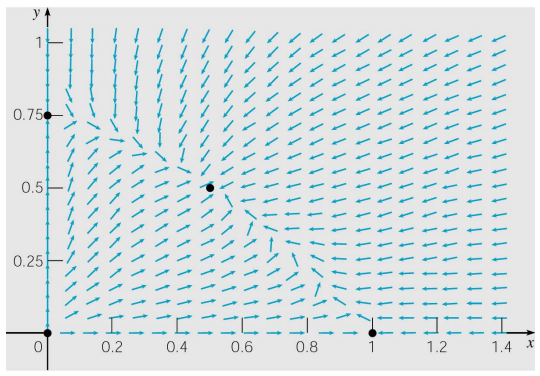
\includegraphics[width=0.55\textwidth]{figure/Lec17f1.PNG}
		\end{figure}
		%
		UCP=unstable critical point\\
		SCP=stable critical point
	\end{itemize}
	%
	\subsection*{Example 1: Direction field (2 of 8)}
	%
	\begin{figure}[H]
		\centering
		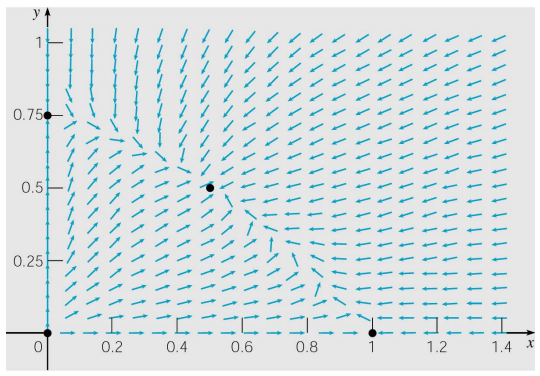
\includegraphics[width=0.75\textwidth]{figure/Lec17f1.PNG}
	\end{figure}
	%
	\subsection*{Example 1: Linearization (3 of 8)}
	\begin{itemize}
		\item Our system of equations,
		$$
		dx/dt = x(1-x-y),\ dy/dt = y(0.75-y-0.5x)
		$$
		is almost linear, since $F$ and $G$ are twice differentiable.
		\item To obtain the linear system near a critical point $(x_0, y_0)$, we use the results of the Lecture 16, given below.
		$$
		\frac{d}{dt} 
		\begin{pmatrix}
			u\\
			v
		\end{pmatrix}=
		\begin{pmatrix}
			F_x(x_0, y_0) & F_y(x_0,y_0)\\
			G_x(x_0,y_0) & G_y(x_0, y_0)
		\end{pmatrix}
		\begin{pmatrix}
			u\\
			v
		\end{pmatrix},\ \text{where}\ 
		\begin{pmatrix}
			x - x_0\\
			y - y_0
		\end{pmatrix}
		$$
		\item Thus
		$$
		\frac{d}{dt}
		\begin{pmatrix}
			u\\
			v
		\end{pmatrix} = 
		\begin{pmatrix}
			1 - 2x_0 - y_0 & -x_0\\
			-0.5y_0 & 0.75 - 2y_0 - 0.5x_0
		\end{pmatrix}
		\begin{pmatrix}
			u\\
			v
		\end{pmatrix}
		$$
	\end{itemize}
	%
	\subsection*{Example 1: Critical point at (0,0) (4 of 8)}
	\begin{itemize}
		\item For the critical point $(0,0)$, the approximating linear system is
		$$
		\frac{d}{dt}
		\begin{pmatrix}
			x\\
			y
		\end{pmatrix}=
		\begin{pmatrix}
			1 & 0\\
			0 & 0.75
		\end{pmatrix}
		\begin{pmatrix}
			x\\
			y
		\end{pmatrix}
		$$
		\item The eigenvalues and eigenvectors are
		$$
		r_1 = 1,\ \xi^{(1)} =
		\begin{pmatrix}
			1\\
			0
		\end{pmatrix};\quad
		r_2 = 0.75\ \xi^{(2)}=
		\begin{pmatrix}
			0\\
			1
		\end{pmatrix}
		$$
		and hence the general solution for this linear system is
		$$
		\begin{pmatrix}
			x\\
			y
		\end{pmatrix} = c_1
		\begin{pmatrix}
			1\\
			0
		\end{pmatrix}e^t + c_2
		\begin{pmatrix}
			0\\
			1
		\end{pmatrix}e^{0.75t}
		$$
		\item Thus the origin is an unstable node of both the linear and nonlinear systems. The trajectories near the origin are all tangent to the y-axis, except for one trajectory that lies along the x-axis.
	\end{itemize}
	%
	\subsection*{Example 1: Critical point at (1,0) (5 of 8)}
	\begin{itemize}
		\item For the critical point $(1,0)$, the approximating linear system is
		$$
		\frac{d}{dt}
		\begin{pmatrix}
			u\\
			v
		\end{pmatrix}=
		\begin{pmatrix}
			-1 & -1\\
			0 & 0.25
		\end{pmatrix}
		\begin{pmatrix}
			u\\
			v
		\end{pmatrix}
		$$
		\item The eigenvalues and eigenvectors are
		$$
		r_1 = -1,\ \xi^{(1)}=
		\begin{pmatrix}
			1\\
			0
		\end{pmatrix};\ 
		r_2 = 0.25,\ \xi^{(2)} =
		\begin{pmatrix}
			4\\
			-5
		\end{pmatrix}
		$$
		and hence the general solution for this linear system is
		$$
		\begin{pmatrix}
			u\\
			v
		\end{pmatrix} = c_1
		\begin{pmatrix}
			1\\
			0
		\end{pmatrix}e^{-t} + c_2
		\begin{pmatrix}
			4\\
			-5
		\end{pmatrix}e^{0.25t}
		$$
		\item Thus $(1,0)$ is an unstable saddle point of both the linear and nonlinear systems. One pair of trajectories approach $(1,0)$ along the x-axis, while all other trajectories depart from $(1,0)$.
	\end{itemize}
	%
	\subsection*{Example 1: Critical point at $(0,0.75)$ (6 of 8)}
	\begin{itemize}
		\item For the critical point $(0,0.75)$, the linear system is
		$$
		\frac{d}{dt} 
		\begin{pmatrix}
			u\\
			v
		\end{pmatrix} =
		\begin{pmatrix}
			0.25 & 0\\
			-0.375 & -0.75
		\end{pmatrix}
		\begin{pmatrix}
			u\\
			v
		\end{pmatrix}
		$$
		\item The eigenvalues and eigenvectors are
		$$
		r_1 = 0.25,\ \xi^{(1)} =
		\begin{pmatrix}
			8\\
			-3
		\end{pmatrix};\ r_2 = -0.75,\ \xi^{(2)}=
		\begin{pmatrix}
			0\\
			1
		\end{pmatrix}
		$$
		and hence the general solution for this linear system is
		$$
		\begin{pmatrix}
			u\\
			v
		\end{pmatrix} = c_1
		\begin{pmatrix}
			8\\
			-3
		\end{pmatrix}e^{0.25t} + c_2
		\begin{pmatrix}
			0\\
			1
		\end{pmatrix}e^{-0.75t}
		$$
		\item Thus $(0,0.75)$ is an unstable saddle point of both the linear and nonlinear systems. One pair of trajectories approach $(0,0.75)$ along y-axis, while all other trajectories depart from $(0,0.75)$.
	\end{itemize}
	%
	\subsection*{Example 1: Critical point at $(0.5,0.5)\ (7 of 8)$}
	\begin{itemize}
		\item For the critical point $(0.5,0.5)$, the linear system is
		$$
		\frac{d}{dt}
		\begin{pmatrix}
			u\\
			v
		\end{pmatrix} =
		\begin{pmatrix}
			-0.5 & -0.5\\
			-0.25 & -0.5
		\end{pmatrix}
		\begin{pmatrix}
			u\\
			v
		\end{pmatrix}
		$$
		\item The eigenvalues and eigenvectors are
		$$
		r_1 = \frac{-2 + \sqrt{2}}{4}\cong -0.146,\ \xi^{(1)} =
		\begin{pmatrix}
			\sqrt{2}\\
			-1
		\end{pmatrix};\ r_2 = \frac{-2 - \sqrt{2}}{4} \cong -0.854,\ \xi^{(2)}=
		\begin{pmatrix}
			\sqrt{2}\\
			1
		\end{pmatrix}
		$$
		and hence the general solution for this linear system is
		$$
		\begin{pmatrix}
			u\\
			v
		\end{pmatrix} = c_1
		\begin{pmatrix}
			\sqrt{2}\\
			-1
		\end{pmatrix}e^{-0.146t} + c_2
		\begin{pmatrix}
			\sqrt{2}\\
			1
		\end{pmatrix}e^{-0.854t}
		$$
		\item Thus $(0.5,0.5)$ is an asymptotically stable node of both the linear and nonlinear systems.
	\end{itemize}
	%
	\subsection*{Example 1: Phase portrait (8 of 8)}
	\begin{itemize}
		\item A phase portrait is given below, along with the direction field, for our nonlinear system
		$$
		dx/dt = x(1-x-y),\ dy/dt = y(0.75 - y - 0.5x)
		$$
		\item Note that the quadratic terms in these equations are all negative, and hence $x^\prime < 0$ and $y^\prime < 0$ for large $x$ and $y$.
		\item Thus the trajectories are directed inward towards $(0.5,0.5)$.
		%
		\begin{figure}[H]
			\centering
			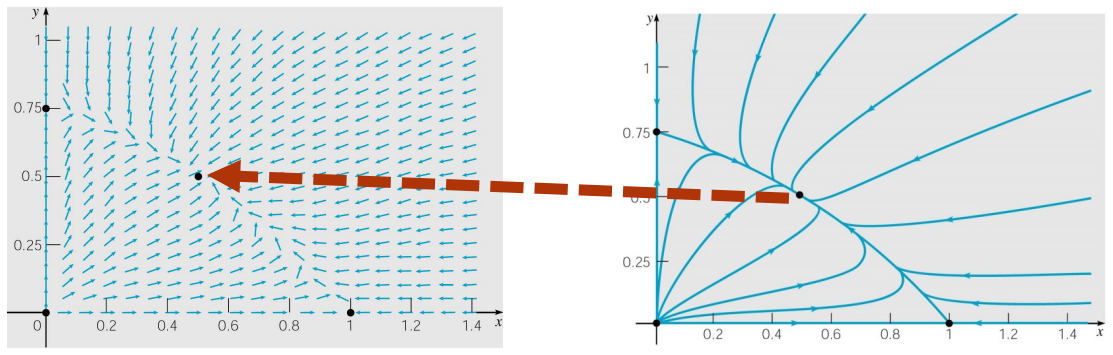
\includegraphics[width=0.85\textwidth]{figure/Lec17f3.PNG}
		\end{figure}
		%
	\end{itemize}
	%
	\subsection*{Population dynamics: Predator-Prey systems}
	\begin{itemize}
		\item In Example 1 we discussed a model of two species that interact by competing for a common food supply or other natural resource.
		\item Here we investigate the situation in which one species (the predator) preys on the other species (the prey), while the prey lives on some other source of food.
		\item For example, foxes and rabbits in a closed forest.
		\item Again we emphasize that a model involving only two species cannot fully describe the complex relationships among species that occur in nature.
		\item Nevertheless, the study of simple models is the first step toward an understanding of more complicated phenomena.
	\end{itemize}
	%
	\subsection*{Assumptions}
	\begin{itemize}
		\item Let $x$ and $y$ be the populations of the prey and predator, respectively, at time $t$.
		\item We make the following assumptions:
		\begin{itemize}
			\item[\labelitemi] In the absence of the predator, the prey grows at a rate proportional to the current population; thus $dx/dt = ax,\ a > 0$, when $y = 0$.
			\item[\labelitemi] In the absence of the prey, the predator dies out at a rate proportional to the current population; thus $dy/dt = -cy,\ c > 0$, when $x = 0$.
			\item[\labelitemi] The number of encounters between predator and prey is proportional to the product of their populations. Each such encounter tends to promote the growth of the predator and to inhibit the growth of the prey. Thus the growth rate of the predator is increased by a term of the form $\gamma xy$, while the growth rate of the prey is decreased by a term $-\alpha xy$, where $\gamma$ and $\alpha$ are positive constants.
		\end{itemize}
	\end{itemize}
	%
	\subsection*{Predator-Prey equations}
	\begin{itemize}
		\item Thus we have the system of equations
		\begin{align*}
			& dx/dt = ax - \alpha\, xy = x(a-\alpha y),\\
			& dy/dt = -cy + \gamma\, xy = y(-c+\gamma x)
		\end{align*}
		\item The constants $a,\ c,\ \alpha,\ \gamma$ are all positive, where $a,\ c$ are the growth rate of prey and death rate of predator, respectively, and $\alpha,\ \gamma$ are measures of the effect of the interaction between the two species.
		\item The predator-prey equations are known as the Lotka-Volterra equations. Although they are rather simple equations, they do characterize a wide class of problems.
		\item Our goal here is to determine the qualitative behavior of the solutions for arbitrary positive initial values of $x$ and $y$.
	\end{itemize}
	%
	\subsection*{Example 2: Population equations (1 of 8)}
	\begin{itemize}
		\item Consider the system of equations
		$$
		dx/dt = x-0.5xy,\ dy/dt = -0.75y + 0.25xy,\quad x,y>0
		$$
		\item The critical points are $(0,0)$ and $(3,2)$.
		\item Given below is a direction field for this system of equations, with the critical points indicated as heavy dots.
		\item The trajectories appear to be closed curves surrounding the critical point $(3,2)$.
		%
		\begin{figure}[H]
			\centering
			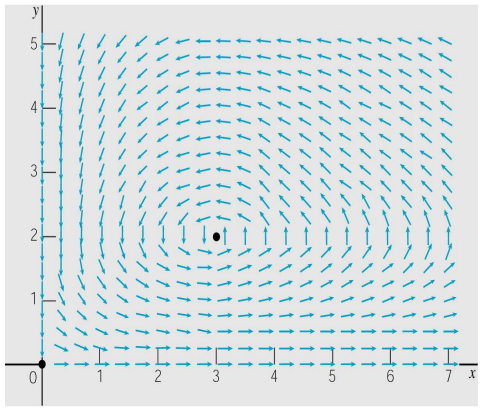
\includegraphics[width=0.55\textwidth]{figure/Lec17f4.PNG}
		\end{figure}
		%
		UCP=unstable critical point\\
		SCP=stable critical point
	\end{itemize}
	%
	\subsection*{Example 2: Population equations (1 of 8)}
	%
	\begin{figure}[H]
		\centering
		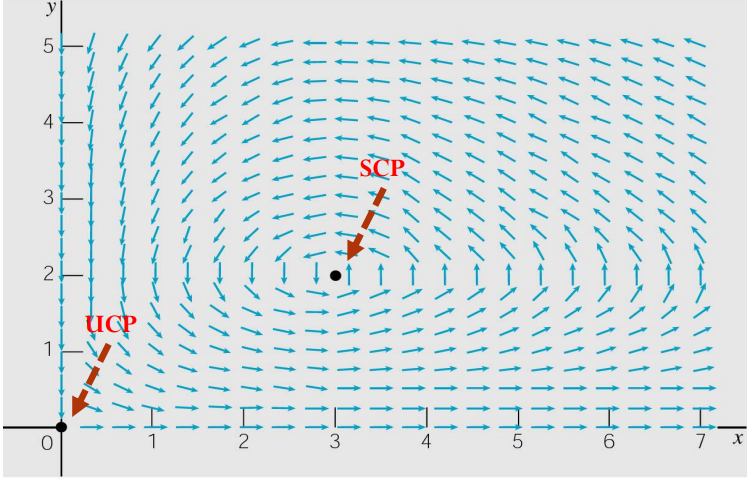
\includegraphics[width=0.85\textwidth]{figure/Lec17f5.PNG}
	\end{figure}
	%
	\subsection*{Example 2: Critical point at $(0,0)$ (2 of 8)}
	\begin{itemize}
		\item For the critical point $(0,0)$, the approximating linear system is
		$$
		\frac{d}{dt}
		\begin{pmatrix}
			x\\
			y
		\end{pmatrix}=
		\begin{pmatrix}
			1 & 0\\
			0 & -0.75
		\end{pmatrix}
		\begin{pmatrix}
			x \\
			y
		\end{pmatrix}
		$$
		\item The eigenvalues and eigenvectors are
		$$
		r_1 = 1,\ \xi^{(1)} =
		\begin{pmatrix}
			1\\
			0
		\end{pmatrix};\ r_2 = -0.75,\ \xi^{(2)}=
		\begin{pmatrix}
			0\\
			1
		\end{pmatrix}
		$$
		and hence the general solution for this linear system is
		$$
		\begin{pmatrix}
			x\\
			y
		\end{pmatrix} = c_1
		\begin{pmatrix}
			1\\
			0
		\end{pmatrix}e^t + c_2
		\begin{pmatrix}
			0\\
			1
		\end{pmatrix}e^{-0.75t}
		$$
		\item Thus $(0,0)$ is an unstable saddle point of both the linear and nonlinear systems. One trajectory approaches $(0,0)$ along the y-axis, while all other trajectories depart from $(0,0)$.
	\end{itemize}
	%
	\subsection*{Example 2: Critical point at $(3,2)$ (3 of 8)}
	\begin{itemize}
		\item For the critical point $(3,2)$, the approximating linear system is
		$$
		\frac{d}{dt}
		\begin{pmatrix}
			u\\
			v
		\end{pmatrix} =
		\begin{pmatrix}
			0 & -1.5\\
			0.5 & 0
		\end{pmatrix}
		\begin{pmatrix}
			u\\
			v
		\end{pmatrix},\quad
		\begin{pmatrix}
			u\\
			v
		\end{pmatrix}=
		\begin{pmatrix}
			x-3\\
			y-2
		\end{pmatrix}
		$$
		\item The eigenvalues and eigenvectors are
		$$
		r_1 = \frac{\sqrt{3}i}{2},\ \xi^{(1)} = 
		\begin{pmatrix}
			1\\
			-i/\sqrt{3}
		\end{pmatrix};\quad r_2 = -\frac{\sqrt{3}i}{2},\ \xi^{(2)} =
		\begin{pmatrix}
			1\\
			i/\sqrt{3}
		\end{pmatrix}
		$$
		\item Thus $(3,2)$ is stable center point of the linear system, but is indeterminate for the nonlinear systems, by Theorem 9.3.2.
		\item To find the trajectories for the linear system, we have
		$$
		\frac{dv/dt}{du/dt} = \frac{dv}{du} = -\frac{0.5u}{1.5v} = -\frac{u}{3v}
		$$
	\end{itemize}
	%
	\subsection*{Example 2: Critical point at $(3,2)$ (4 of 8)}
	\begin{itemize}
		\item Near the critical point $(3,2)$, we thus have
		$$
		dv/du = -u/3v
		$$
		\item The solution to this separable equation is
		$$
		u^2 + 3v^2 = k,\ k>0
		$$
		\item Thus the trajectories of the linear system are ellipses centered at the critical point $(3,2)$, and are elongated horizontally.
		\item Returning to the nonlinear system
		$$
		dx/dt = x-0.5xy,\ dy/dt = -0.75y+0.25xy,\quad x,y>0
		$$
		we have
		$$
		\frac{dy}{dx} = \frac{-0.75y+0.25xy}{x-0.5xy}
		$$
	\end{itemize}
	%
	\subsection*{Example 2: Critical point at (3,2) (5 of 8)}
	\begin{itemize}
		\item Thus
		$$
		\frac{dy}{dx} = \frac{y(-0.75 + 0.25x)}{x(1-0.5y)} \Leftrightarrow \frac{1-0.5y}{y}dy = \frac{-0.75 + 0.25x}{x}dx
		$$
		\item The solution to this separable equation is
		$$
		0.75\ln x + \ln y - 0.5y - 0.25x = c
		$$
		\item It can be shown that the graph of this equation, for a fixed $c$, is a closed curve about the point $(3,2)$.
		\item Thus the critical point $(3,2)$ is also a center of our nonlinear system, and hence the predator and prey populations exhibit a cyclic variation about the equilibrium solution $(3,2)$.
		\item This behavior is seen in the phase portrait on the next slide.
	\end{itemize}
	%
	\subsection*{Example 2: Phase portrait (6 of 8)}
	\begin{itemize}
		\item Given below is a phase portrait for our nonlinear system.
		\item For some initial conditions, the trajectories represent small variations in $x$ and $y$ about $(3,2)$, and are almost elliptical in shape, as the linear analysis suggests.
		\item For other initial points, the oscillations in $x$ and $y$ are more pronounced, and the shape of the trajectories are significantly different from an ellipse.
		\item Note that the trajectories are traversed counterclockwise.
		%
		\begin{figure}[H]
			\centering
			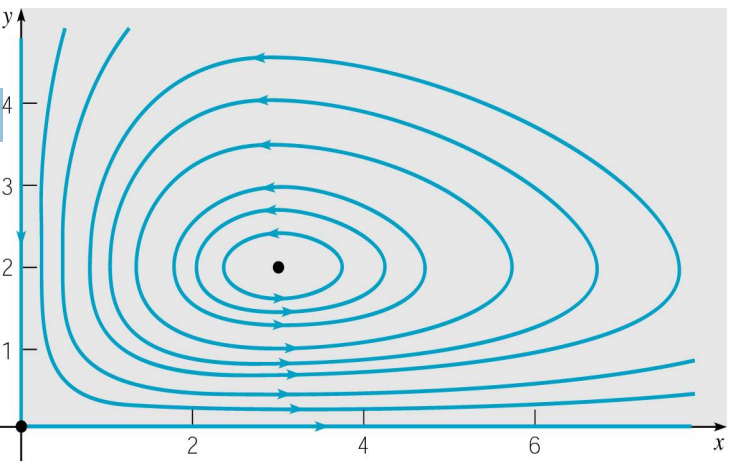
\includegraphics[width=0.55\textwidth]{figure/Lec17f6.PNG}
		\end{figure}
		%
	\end{itemize}
	%
	\subsection*{Example 2: Population equations (7 of 8)}
	\begin{itemize}
		\item A phase portrait along with population graphs $x(t)$ and $y(t)$, for a typical set of initial conditions, are given below.
		\item Note from both of these figures that the oscillation of the predator population lags behind that of the prey.
		%
		\begin{figure}[H]
			\centering
			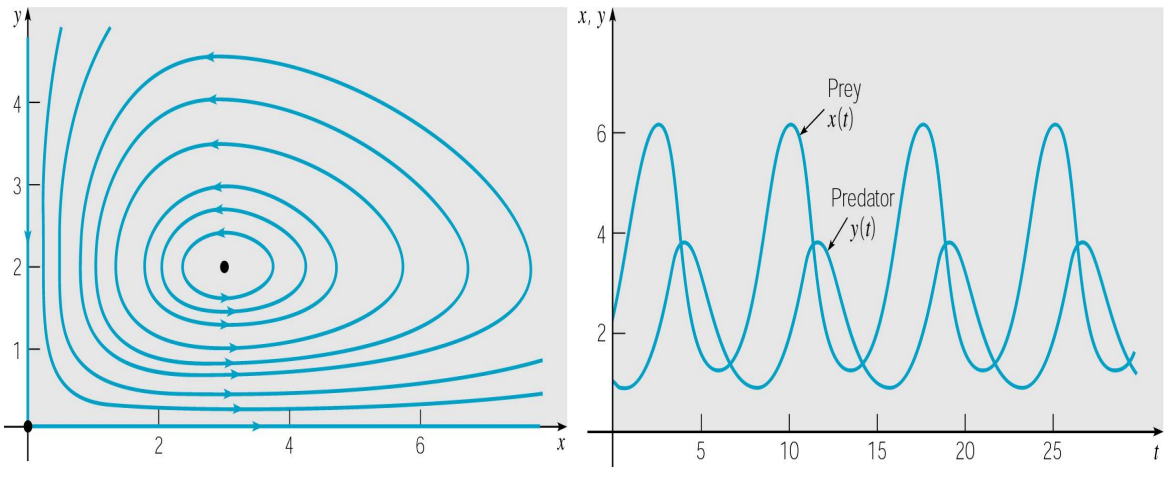
\includegraphics[width=0.85\textwidth]{figure/Lec17f7.PNG}
		\end{figure}
		%
	\end{itemize}
	%
	\subsection*{Example 2: Population equations (8 of 8)}
	\begin{itemize}
		\item Starting with a state in which both populations are relatively small, the prey first increase because of little predation.
		\item Then the predators, with abundant food, increase in population.
		\item This causes heavy predation, and the prey tend to decrease.
		\item Finally, with a diminished food supply, the predator population also decreases, and the system returns to original state.
		%
		\begin{figure}[H]
			\centering
			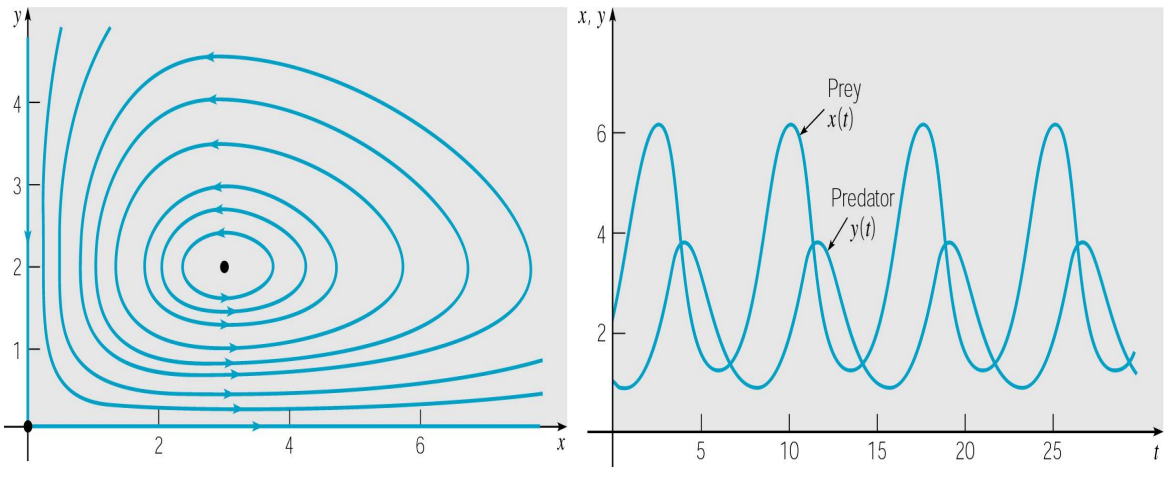
\includegraphics[width=0.85\textwidth]{figure/Lec17f7.PNG}
		\end{figure}
		%
	\end{itemize}
\end{document}